\section{探索性数据分析}
    \begin{enumerate}
        \item
        \code
\begin{lstlisting}
w <- c(72,61,72,61,66,61,80,
       71,80,80,72,71,67,61,
       76,68,68,73,81,66,75,
       75,61,76,91,96,86)
# 求均值
w.mean <- mean(w); w.mean
# 求中位数
w.median <- median(w); w.median
# 求分位数
q.quantile = quantile(w); q.quantile
# 求下四分位数
Q1 = q.quantile[2]; Q1
# 求上四分位数
Q3 = q.quantile[4]; Q3
# 求三均值
M3 = Q1*(1/4) + q.quantile[3]*(1/2) + Q3*(1/4); M3
\end{lstlisting}
        \out
\begin{lstlisting}
> # 求均值
> w.mean <- mean(w); w.mean
[1] 72.85185
> # 求中位数
> w.median <- median(w); w.median
[1] 72
> # 求分位数
> q.quantile = quantile(w); q.quantile
  0%  25%  50%  75% 100% 
61.0 66.5 72.0 78.0 96.0 
> # 求下四分位数
> Q1 = q.quantile[2]; Q1
 25% 
66.5 
> # 求上四分位数
> Q3 = q.quantile[4]; Q3
75% 
 78 
> # 求三均值
> M3 = Q1*(1/4) + q.quantile[3]*(1/2) + Q3*(1/4); M3
   25% 
72.125 
\end{lstlisting}
        \summary\\
        均值为72.85185;中位数为72;下四分位数为66.5;上四分位数为78.0;三均值为72.125。
        \item
        \code
\begin{lstlisting}
w <- c(72,61,72,61,66,61,80,
       71,80,80,72,71,67,61,
       76,68,68,73,81,66,75,
       75,61,76,91,96,86)
m <- mean(w); m
# 求方差
v <- var(w); v
# 求标准差
s <- sd(w); s
# 求极差
R <- max(w) - min(w); R
# 求变异系数
cv <- (s/m); cv
# 求四分位极差
q.quantile = quantile(w)
Q1 = q.quantile[2]
Q3 = q.quantile[4]
R1 <- Q3 - Q1; R1
# 求上截断点
Qu <- Q3 + 1.5*R1; Qu
# 求下截断点
Qd <- Q1 - 1.5*R1; Qd
\end{lstlisting}
        \out
\begin{lstlisting}
> m <- mean(w); m
[1] 72.85185
> # 求方差
> v <- var(w); v
[1] 83.59259
> # 求标准差
> s <- sd(w); s
[1] 9.142898
> # 求极差
> R <- max(w) - min(w); R
[1] 35
> # 求变异系数
> cv <- (s/m); cv
[1] 0.1254999
> # 求四分位极差
> q.quantile = quantile(w)
> Q1 = q.quantile[2]
> Q3 = q.quantile[4]
> R1 <- Q3 - Q1; R1
 75% 
11.5 
> # 求上截断点
> Qu <- Q3 + 1.5*R1; Qu
  75% 
95.25 
> # 求下截断点
> Qd <- Q1 - 1.5*R1; Qd
  25% 
49.25 
\end{lstlisting}
        \summary\\
        方差为83.59259;标准差为9.142898;极差为35;变异系数为0.1254999;四分位极差为11.5;上截断点为95.25;下截断点为49.25。
        \item
        \code
\begin{lstlisting}
source("summarize.R")
w <- c(72,61,72,61,66,61,80,
       71,80,80,72,71,67,61,
       76,68,68,73,81,66,75,
       75,61,76,91,96,86)
summarize(w)
\end{lstlisting}
        \out
\begin{lstlisting}
> summarize(w)
   N     Mean      Var  std_dev Median        CV      CSS    USS     M3  R   R1
1 27 72.85185 83.59259 9.142898     72 0.1254999 2173.407 145473 72.125 35 11.5
   Skewness  Kurtosis
1 0.7044859 0.3881179
\end{lstlisting}
        \summary\\
        数量为27;均值为72.85185;方差为83.59259;标准差为9.142898;中位数为72;变异系数为0.1254999;样本校正平方和为2173.407;样本未校正平方和为145473;三均值为72.125;极差为35;四分位极差为11.5;偏度系数为0.7044859;峰度系数为0.3881179。
        \item
        \code
\begin{lstlisting}
w <- scan("ex1_4-data.txt")
# 绘制密度直方图
hist(w, freq=FALSE, xlim = c(2,8), ylim = c(0,0.6))
# 绘制密度估计曲线
lines(density(w), type="l")
x <- 2:8
# 绘制正态分布概率密度曲线
lines(x, dnorm(x, mean(w), sd(w)), type="b")
\end{lstlisting}
        \out
        \begin{figure}[H]
            \centering
            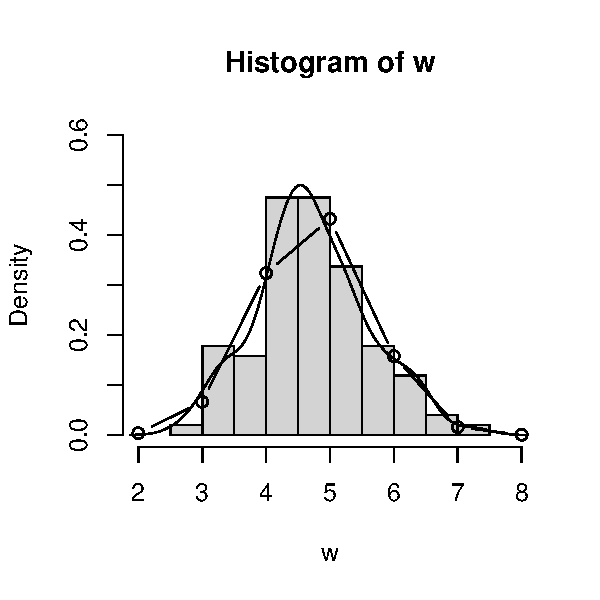
\includegraphics[scale=0.7]{1-4.pdf}
            \caption{题4图}
        \end{figure}
        \summary\\
        由线条显示的曲线是密度估计曲线,而点和线交错显示的曲线是相应正态分布的概率密度曲线。密度估计曲线与正态分布的概率密度曲线有一定差别,但不是很大,可近似认为样本符合正态分布。
        \item
        \code
\begin{lstlisting}
w <- scan("ex1_5-data.txt")
# 绘制茎叶图
stem(w)
# 绘制箱线图
boxplot(w)
# 计算五数总括
fivenum(w)
\end{lstlisting}
        \out
\begin{lstlisting}
> stem(w)

  The decimal point is at the |

  12 | 069
  14 | 477901112223336899
  16 | 0111233446677902233345555567789
  18 | 001223338891123355579
  20 | 0005689003588
  22 | 089
  24 | 346816
  26 | 
  28 | 
  30 | 0
\end{lstlisting}
        \begin{figure}[H]
            \centering
            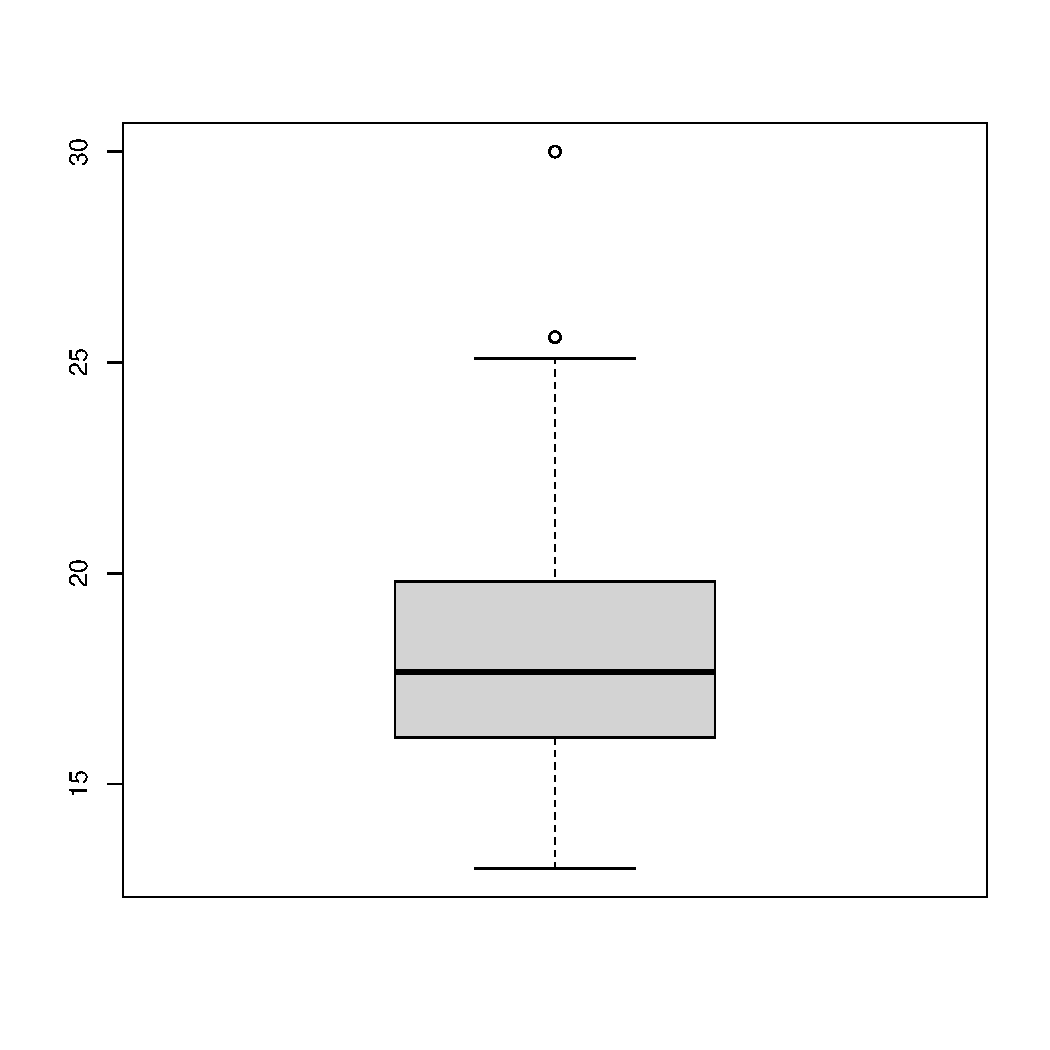
\includegraphics[scale=0.5]{1-5箱线图.pdf}
            \caption{题5箱线图}
        \end{figure}
\begin{lstlisting}
> fivenum(w)
[1] 13.00 16.10 17.65 19.80 30.00
\end{lstlisting}
        \summary
        \begin{enumerate}[label=(\arabic*)]
            \item 从茎叶图可以看出,绝大部分数据集中在$14 \sim 20$,在$16 \sim 18$形成一个高峰;数据分布不对称,有异常数据30.0;
            \item 从箱线图可以看出,数据存在异常值30.0,集中在较大值一侧,分布呈右偏态;
            \item 五数总括中,最小值为13.00,下四分位数为16.10,中位数为17.65,上四分位数为19.80,最大值为30.00。
        \end{enumerate}
        \item
        \code
\begin{lstlisting}
w <- scan("ex1_5-data.txt")
# 绘制经验分布函数曲线
plot(ecdf(w), verticals=TRUE, do.p=FALSE)
x <- 12:31
# 绘制正态分布函数曲线
lines(x, pnorm(x, mean(w), sd(w)))
\end{lstlisting}
        \out
        \begin{figure}[H]
            \centering
            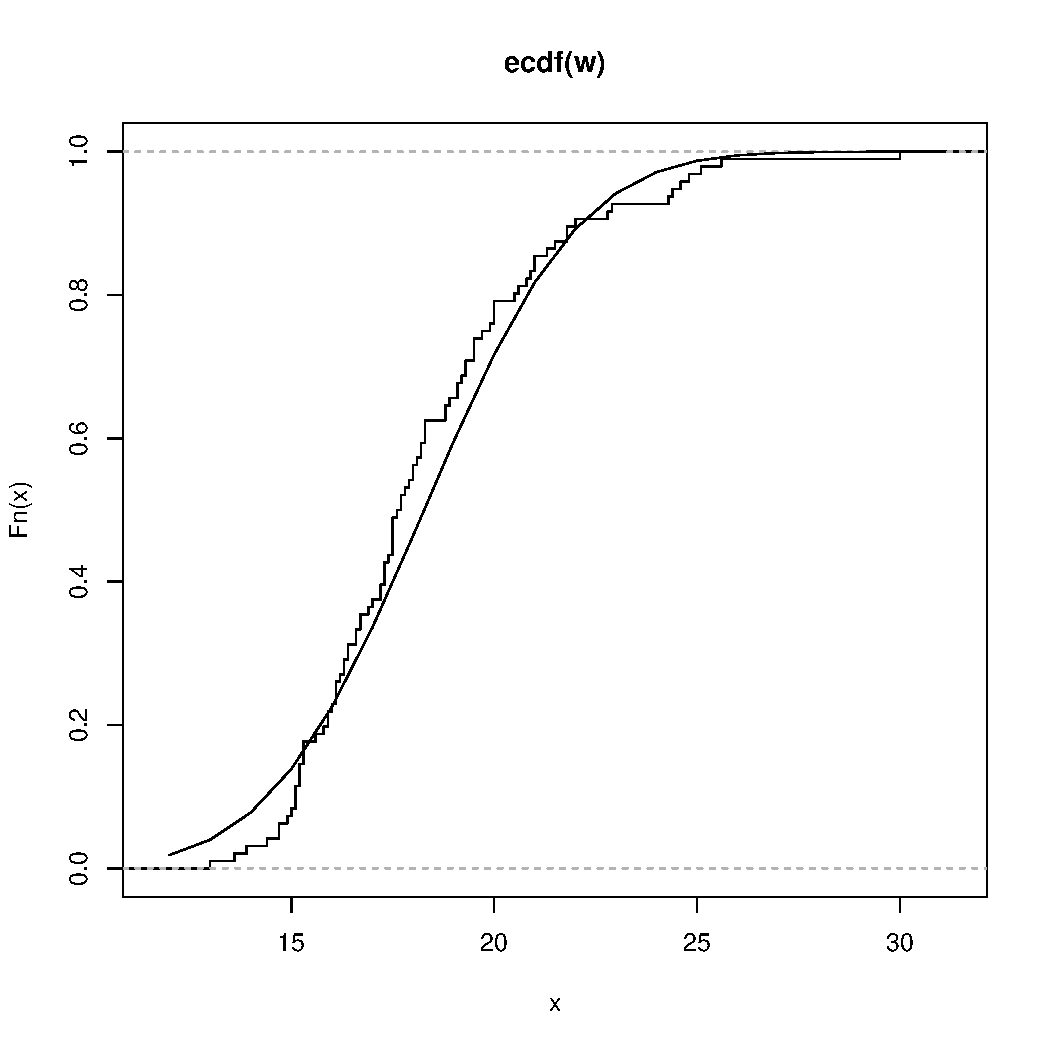
\includegraphics[scale=0.5]{1-6.pdf}
            \caption{题6图}
        \end{figure}
        \summary\\
        儿童体重的经验分布函数曲线用正态分布函数曲线拟合效果良好,可以认为数据来自正态总体。
        \item
        \code
\begin{lstlisting}
w <- scan("ex1_5-data.txt")
# 绘制正态QQ图
qqnorm(w)
qqline(w)
\end{lstlisting}
        \clearpage
        \out
        \begin{figure}[H]
            \centering
            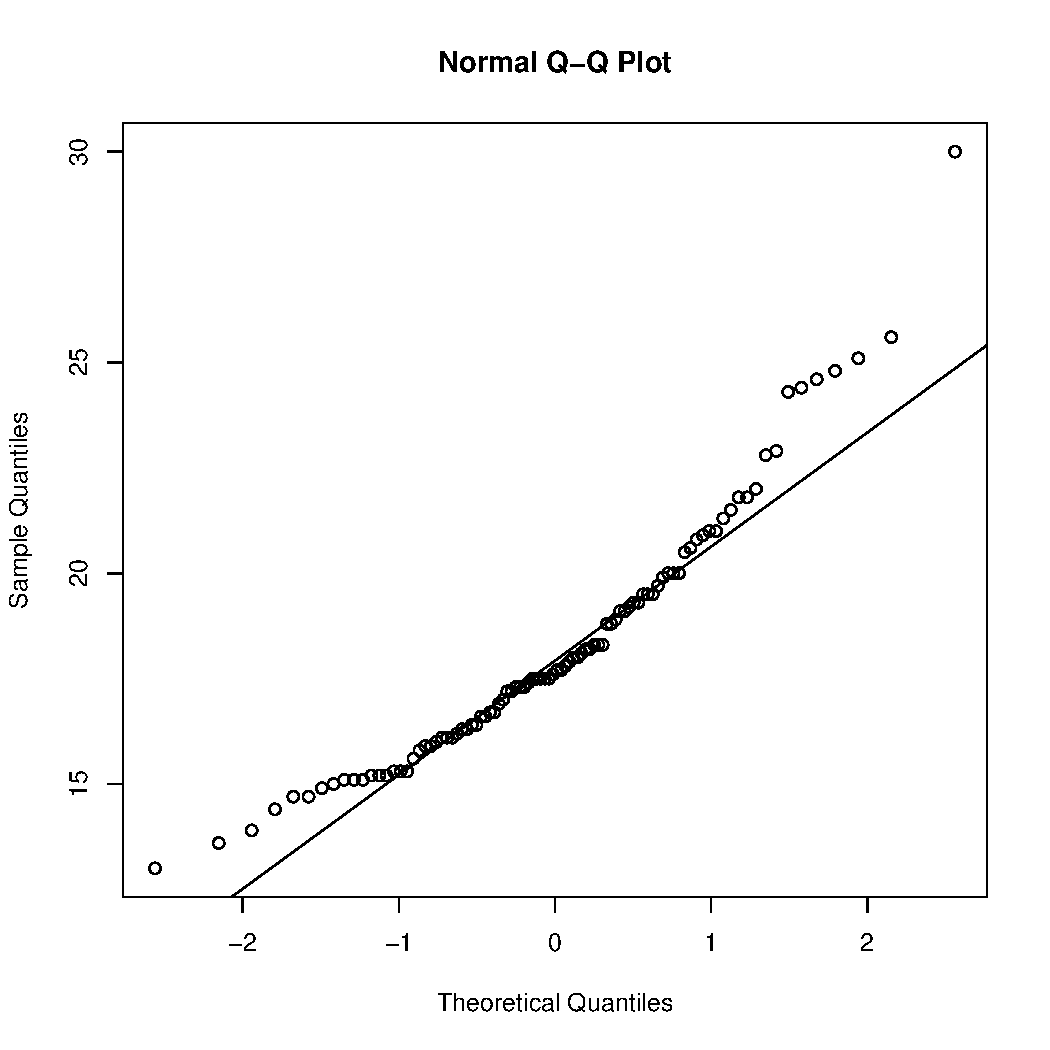
\includegraphics[scale=0.5]{1-7.pdf}
        \end{figure}
        \summary\\
        这些点中间部分近似在一条直线上,但首尾偏差较大,无法认为样本数据来自正态总体。
        \item
        \code
\begin{lstlisting}
w <- scan("ex1_5-data.txt")
n <- length(w);
k <- floor(1+3.3*log10(n));
R <- max(w) - min(w);
d <- round(R/k); d
A <- table(cut(w, br=c(13,15,17,19,21,23,30))); A
p <- pnorm(c(15,17,19,21,23,30), mean(w), sd(w));
p <- c(p[1],p[2]-p[1],p[3]-p[2],p[4]-p[3],p[5]-p[4],1-p[5]); p
chisq.test(A, p=p)
\end{lstlisting}
        \out
\begin{lstlisting}
> d <- round(R/k); d
[1] 2
> A <- table(cut(w, br=c(13,15,17,19,21,23,30))); A

(13,15] (15,17] (17,19] (19,21] (21,23] (23,30] 
      7      28      27      19       7       7 
> p <- c(p[1],p[2]-p[1],p[3]-p[2],p[4]-p[3],p[5]-p[4],1-p[5]); p
[1] 0.13841648 0.19775300 0.25927817 0.22211154 0.12430578 0.05813504
> chisq.test(A, p=p)

	Chi-squared test for given probabilities

data:  A
X-squared = 10.185, df = 5, p-value = 0.07016
\end{lstlisting}
        \summary\\
        $H_0:$来自正态总体,$H_1:$不来自正态总体,$p$值$= 0.07016 > 0.05$,则接受原假设,认为数据来自正态总体。
        \item
        \code
\begin{lstlisting}
red <- seq(420, 640, by = 20)
num <- c(2,4,7,16,20,20,24,22,16,2,6,1)
w <- rep(red, num)
ks.test(w, "pnorm", mean(w), sd(w))
\end{lstlisting}
        \out
\begin{lstlisting}
> ks.test(w, "pnorm", mean(w), sd(w))

	One-sample Kolmogorov-Smirnov test

data:  w
D = 0.10583, p-value = 0.0869
alternative hypothesis: two-sided

Warning message:
In ks.test(w, "pnorm", mean(w), sd(w)) :
  Kolmogorov - Smirnov检验里不应该有连结
\end{lstlisting}
        \summary\\
        $H_0:$数据来自正态总体,$H_1:$数据不是来自正态总体,$p$值为$0.0869>0.05$,则接受原假设,认为数据来自正态总体。
        \item
        \code
\begin{lstlisting}
w <- c(0.54,0.81,0.87,0.21,0.31,
       0.40,0.46,0.17,0.62,0.63,
       0.99,0.71,0.14,0.12,0.64,
       0.51,0.68,0.50,0.60,0.78)
# X^2拟合优度检验
A <- table(cut(w, br=c(0,0.2,0.4,0.6,0.8,1))); A
p <- punif(c(0.2,0.4,0.6,0.8,1), 0, 1);
p <- c(p[1],p[2]-p[1],p[3]-p[2],p[4]-p[3],1-p[4]); p
chisq.test(A, p=p)
# K-S检验
ks.test(w, "punif", 0, 1)
\end{lstlisting}
        \out
\begin{lstlisting}
> # X^2拟合优度检验
> A <- table(cut(w, br=c(0,0.2,0.4,0.6,0.8,1))); A

  (0,0.2] (0.2,0.4] (0.4,0.6] (0.6,0.8]   (0.8,1] 
        3         3         5         6         3 
> p <- c(p[1],p[2]-p[1],p[3]-p[2],p[4]-p[3],1-p[4]); p
[1] 0.2 0.2 0.2 0.2 0.2
> chisq.test(A, p=p)

	Chi-squared test for given probabilities

data:  A
X-squared = 2, df = 4, p-value = 0.7358

Warning message:
In chisq.test(A, p = p) : Chi-squared近似算法有可能不准
> # K-S检验
> ks.test(w, "punif", 0, 1)

	One-sample Kolmogorov-Smirnov test

data:  w
D = 0.16, p-value = 0.6285
alternative hypothesis: two-sided
\end{lstlisting}
        \summary
        \begin{enumerate}[label=(\arabic*)]
            \item $H_0:$来自$[0,1]$上的均匀分布,$H_1:$不来自$[0,1]$上的均匀分布,$\chi^2$拟合优度检验的$p$值为$0.7358>0.05$,则接受原假设,认为数据来自$[0,1]$上的均匀分布。
            \item $H_0:$来自$[0,1]$上的均匀分布,$H_1:$不来自$[0,1]$上的均匀分布,K-S检验的$p$值为$0.6285>0.05$,则接受原假设,认为数据来自$[0,1]$上的均匀分布。
        \end{enumerate}
        \item
        \code
\begin{lstlisting}
w <- c(36,32,16,15,35)
p <- c(0.2,0.2,0.2,0.2,0.2)
chisq.test(w, p=p)
\end{lstlisting}
        \out
\begin{lstlisting}
> chisq.test(w, p=p)

	Chi-squared test for given probabilities

data:  w
X-squared = 16.224, df = 4, p-value = 0.002733
\end{lstlisting}
        \summary\\
        $H_0:$不合格率相同,$H_1:$不合格率不相同,$p$值为$0.002733<0.05$,则拒绝原假设,认为五个工作日的产品不合格率不相同。
        \item
        \code
\begin{lstlisting}
w <- c(36,32,16,15,35)
p <- c(0.3,0.25,0.1,0.1,0.25)
chisq.test(w, p=p)
\end{lstlisting}
        \out
\begin{lstlisting}
> chisq.test(w, p=p)

	Chi-squared test for given probabilities

data:  w
X-squared = 1.2687, df = 4, p-value = 0.8667
\end{lstlisting}
        \summary\\
        $H_0:$这种说法正确,$H_1:$这种说法不正确,$p$值为$0.8667>0.05$,则接受原假设,认为这种说法正确。
    \end{enumerate}
\clearpage